\chapter{String phenomenology: from the heterotic string to the moduli problem}
\label{ch:L2}
\lecturedate{Lecture of 6 November 2026}

This lecture continues the general description, begun in \cref{ch:L1}, of how string theory can be connected with the real world; like the first, it is mostly qualitative. It has three parts. The first explains why we look for compactifications that preserve four-dimensional $\mathcal N=1$ supersymmetry at the Kaluza--Klein scale. The second surveys the five superstring theories in ten dimensions, the dualities that relate them and their massless spectra, and uses them to explain why string phenomenology started with the heterotic string and why it later moved to type II theories. The third introduces a problem that every string compactification has to face, and around which much of this course is organised: the \emph{moduli}, massless scalar fields that parametrise the size and the shape of the extra dimensions, and the need to stabilise them.

\section{Why four-dimensional \texorpdfstring{$\mathcal N=1$}{N=1} supersymmetry}
\label{sec:L2-N1}

In the chain of effective theories of \cref{sec:L1-hierarchy} (\cref{fig:L1-scales}), type IIB string theory gives type IIB supergravity below the string scale, and a four-dimensional supergravity below the Kaluza--Klein scale, once the Kaluza--Klein towers (\cref{sec:L1-KK}) are integrated out; how many supersymmetries survive depends on the topology of $Y_6$ (\cref{sec:L1-holonomy}). We pick Calabi--Yau manifolds, to be defined properly later, because they break the largest amount of supersymmetry while preserving some of it, and, after the orientifold projection, lead to $\mathcal N=1$ at the Kaluza--Klein scale.

One could also consider compactifications that break supersymmetry completely, with $\mathcal N=0$ at the Kaluza--Klein scale, and do model building directly there. We do not, for four reasons.

The first is that $\mathcal N=1$ is the only chiral version of four-dimensional supersymmetry: in theories with $\mathcal N\ge2$ the fermions come in non-chiral representations (\cref{sec:L1-holonomy}). With $\mathcal N=1$ there is hope of obtaining the Standard Model, which is a chiral theory.

The second concerns the scale of supersymmetry breaking. The Kaluza--Klein scale is not known: it could be close to the TeV scale, at the edge of detection, but more realistically it is very high, say $10^{14}$--$10^{15}\GeV$. The $\mathcal N=1$ supersymmetry that survives there should then be broken spontaneously at much lower energies, for example at the TeV scale, to address the hierarchy problem, and \emph{dynamically}: the hope is that non-perturbative effects, as in confinement, generate a scale exponentially smaller than the fundamental ones. Supersymmetry broken at low energies has the good properties met in the supersymmetry course: it addresses the hierarchy problem, provides a dark matter candidate, leads to radiative electroweak symmetry breaking, in which loop corrections break the electroweak symmetry dynamically, and makes the gauge couplings unify. The hope is to recover all of these from a top-down approach. Whether this works is a property of the effective theory: one has to derive it from string theory, compute the non-perturbative effects, and check whether they break the remaining $\mathcal N=1$ at low energies. It might also turn out that this is never possible.

The third concerns how the breaking is communicated. Besides knowing whether supersymmetry is broken at low energies, one must understand how the breaking is mediated to the \emph{visible sector}, the supersymmetric version of the Standard Model, for instance the minimal supersymmetric Standard Model (MSSM). Some other sector of the compactification is responsible for breaking supersymmetry, and it must couple to the MSSM in such a way that the MSSM feels the breaking and the supersymmetric partners become massive. The breaking felt by the MSSM must be \emph{soft}, so that the cancellation of quadratic divergences survives, and soft supersymmetry breaking is generated naturally in supergravity theories derived from string theory, through gravitational interactions. This is \emph{gravity mediation}.

These three reasons are phenomenological. The fourth is theoretical, and we have not met it yet in the supersymmetry course: \emph{$\mathcal N=1$ supersymmetry allows one to control the quantum corrections to the effective theory.} A supersymmetric theory is specified by its Kähler potential $K$ and its superpotential $W$, and one can ask how these quantities behave under quantum corrections. Each of them has a tree-level part, loop corrections and non-perturbative corrections, but not on the same footing:
\begin{equation}
  K = K_{\text{tree}} + K_{\text{loops}} + K_{\text{np}} ,\qquad
  W = W_{\text{tree}} + W_{\text{np}} .
  \label{eq:L2-KW}
\end{equation}
The superpotential is exact at tree level in perturbation theory: as a consequence of supersymmetry and of holomorphy it receives no loop corrections, only non-perturbative ones (this will be proved in the supersymmetry course). This is a very powerful result: once $W$ is computed at tree level, one knows for sure that there are no loop corrections. The Kähler potential, instead, does receive loop corrections. Since computing quantum corrections in string theory is extremely hard, this control is very important, and in a compactification that breaks supersymmetry completely it is absent. Keeping some supersymmetry helps to compute the effective theory, but not too much of it: with $\mathcal N=1$, and not $\mathcal N=2$, the theory remains chiral and good for phenomenology. That is the balance.

In an $\mathcal N=0$ compactification a ten-dimensional Majorana--Weyl spinor corresponds to no spinor at all in four dimensions, so a ten-dimensional supersymmetry generator gives nothing. An example is $Y_6 = S^6$, a six-dimensional sphere, whose holonomy group is $SU(4)$ in the lecture's words, to be compared with $SU(3)$ for a Calabi--Yau manifold.
Why the holonomy group determines the number of four-dimensional supersymmetries will be explained towards the end of the course.

\section{Five superstring theories and their dualities}
\label{sec:L2-dualities}

Our starting point will be ten-dimensional type IIB string theory, because, as we shall try to explain, it is at present the most promising one for phenomenology. In the end the starting point does not matter much, since all string theories are related by dualities. What changes from one description to another is which quantities are easy to compute: something that looks weakly coupled, and so computable, in one description can look strongly coupled, and hard to compute, in another.

The five consistent perturbative superstring theories recalled in \cref{sec:L1-aims}, type IIA, type IIB, type I and the two heterotic theories, with gauge groups $SO(32)$ and $E_8\times E_8$, are all related by dualities of two kinds. \emph{S-dualities} are strong--weak coupling dualities: they act on the dilaton, and exchange a theory at string coupling $g_s$ with one at coupling $1/g_s$. \emph{T-dualities} act instead on the geometry: they change the radius of the compactification manifold. The five theories are therefore best thought of not as different theories but as different limits, or better different perturbative corners, of a single, more fundamental theory, \emph{M-theory}. What we know of M-theory is its low-energy limit, eleven-dimensional supergravity. In it, the size of the eleventh dimension corresponds to the string coupling. In a perturbative corner, where the coupling goes to zero and perturbation theory can be used, the size of the eleventh dimension goes to zero, and one recovers a ten-dimensional theory; when the coupling becomes large, one starts to see the eleventh dimension.

The simplest example is the relation between M-theory and type IIA. Compactified on a circle $S^1$ of radius $R$, going from eleven to ten dimensions, M-theory gives type IIA string theory, and $R$ is set by the dilaton in such a way that
\begin{equation}
  R\to0 \qquad\Longleftrightarrow\qquad g_s\to0 \qquad\text{(type IIA limit)} .
  \label{eq:L2-IIA-limit}
\end{equation}
Type IIA is in turn T-dual to type IIB. T-duality changes the size of the compactification manifold: type IIA compactified on a circle of radius $R$ is the same theory as type IIB compactified on a circle of radius
\begin{equation}
  \tilde R = \frac{\alpha'}{R} = \frac{1}{4\pi^2\Ms^2R} .
  \label{eq:L2-Tduality}
\end{equation}
The two are the same theory, with $R$ exchanged for $\alpha'/R$: an example of a duality. The whole web of dualities is shown in \cref{fig:L2-dualities}.

\begin{figure}[tbp]
  \centering
  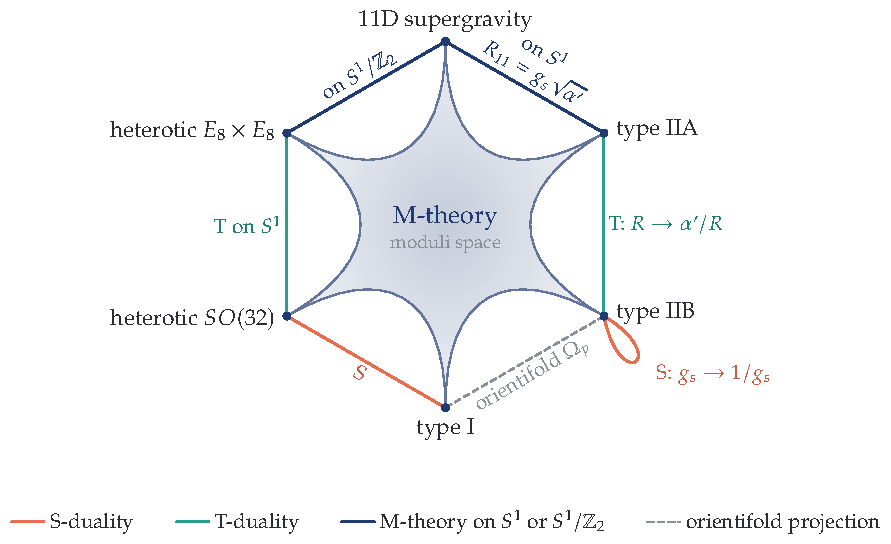
\includegraphics{fig_L2-dualities}
  \caption{The five ten-dimensional superstring theories and eleven-dimensional supergravity as limits of a single theory, M-theory, and the dualities that relate them.}\label{fig:L2-dualities}
\end{figure}

\section{Massless spectra and the first string models}
\label{sec:L2-spectra}

String phenomenology, the attempt to obtain the real world from string theory, started in the mid-1980s: string theory was born at the end of the 1960s and developed in the 1970s, and in the mid-1980s people started trying to connect it with the real world.

These first attempts used not type IIB but the $E_8\times E_8$ heterotic string. The type II theories seemed to give no non-abelian gauge bosons in four dimensions, which are needed for the Standard Model, and so, although consistent, they seemed unfit for the real world. The heterotic string, instead, has a gauge group in its massless spectrum, $E_8\times E_8$, and $E_8$ is a huge group which contains the Standard Model gauge group. The idea was to break one $E_8$ factor down to the Standard Model with a Higgs mechanism, and to use the dynamics of the other to break supersymmetry. This programme turned out to be very hard, for reasons explained below, although heterotic phenomenology is still pursued today. Around 1995 came the discovery of \emph{D-branes} as dynamical objects of string theory, and with it the realisation that the open strings ending on them can behave as non-abelian gauge bosons (\cref{sec:L4-gauge}). D-branes are present in type II theories, so one had simply missed an ingredient: the non-abelian gauge bosons are absent from the closed-string spectrum, but they can come from open strings. Since then type II theories have been studied more than the heterotic string for phenomenology.

To see why, we list the massless modes of the closed string and the ten-dimensional fields they correspond to, in \cref{tab:L2-spectra}, for type IIA, type IIB and the heterotic string.

\begin{table}[tbp]
  \centering
  \renewcommand{\arraystretch}{1.35}
  \begin{tabular}{@{}llll@{}}
    \toprule
    Sector & Type IIA & Type IIB & Heterotic \\
    \midrule
    NS--NS & $G_{MN},\ B_{MN},\ \phi$ & $G_{MN},\ B_{MN},\ \phi$ & $G_{MN},\ B_{MN},\ \phi,\ A^a_M$ \\
    R--R   & $C_1,\ C_3$ & $C_0,\ C_2,\ C_4$ & --- \\
    NS--R  & $\psi^1_{M+},\ \lambda^1_-$ & $\psi^1_{M+},\ \lambda^1_-$ & $\psi_{M+},\ \lambda_-,\ \lambda^a_+$ \\
    R--NS  & $\psi^2_{M-},\ \lambda^2_+$ & $\psi^2_{M+},\ \lambda^2_-$ & --- \\
    \midrule
    10D supersymmetry & $\mathcal N=2$, non-chiral & $\mathcal N=2$, chiral & $\mathcal N=1$, chiral \\
    \bottomrule
  \end{tabular}
  \caption{Massless spectra of the type IIA, type IIB and heterotic superstrings in ten dimensions, sorted by sector: the first label refers to the left-movers, the second to the right-movers (for the heterotic string see the text). $G_{MN}$ is the metric, $B_{MN}$ the Kalb--Ramond two-form, $\phi$ the dilaton, $C_p$ the R--R $p$-forms, $\psi_M$ the gravitini, $\lambda$ the dilatini; $A^a_M$ and $\lambda^a$ are the heterotic gauge bosons and gaugini, $a = 1,\dots,\dim G = 496$, with $G = SO(32)$ or $E_8\times E_8$. The subscripts $\pm$ give the ten-dimensional chirality.}
  \label{tab:L2-spectra}
\end{table}

The labels NS and R stand for Neveu--Schwarz and Ramond, and they are boundary conditions for the fermions on the worldsheet. The bosonic coordinates $X^M(\sigma)$ of a closed string must come back to themselves when one goes around the string, $\sigma\to\sigma+2\pi$. When the theory is supersymmetrised one must add worldsheet fermions $\psi^M$, and these can come back either to themselves or to minus themselves:
\begin{equation}
  \psi^M(\sigma+2\pi) = +\psi^M(\sigma)\quad\text{(Ramond)} ,\qquad
  \psi^M(\sigma+2\pi) = -\psi^M(\sigma)\quad\text{(Neveu--Schwarz)} .
  \label{eq:L2-NSR}
\end{equation}
On a closed string there are left-movers and right-movers, and the condition can be chosen independently for each. In type II theories there are worldsheet fermions for both, and so two spacetime supersymmetries, one coming from the left-movers and one from the right-movers; this is why they are called type II, and why all four combinations NS--NS, R--R, NS--R and R--NS appear. In the heterotic string there are worldsheet fermions only for the right-movers, and so only one spacetime supersymmetry. The left-movers have no worldsheet fermions at all: they are those of the bosonic string. Being bosonic, they produce only spacetime bosons, as an NS sector does, which is why the two heterotic sectors are labelled NS--NS and NS--R, according to the boundary condition of the right-movers.

Now the fields. The NS--NS sector always contains the metric $G_{MN}$, the antisymmetric Kalb--Ramond two-form $B_{MN}$ and the dilaton $\phi$, the spectrum of any bosonic string theory. The heterotic string has in addition gauge bosons $A^a_M$, ten-dimensional vectors (hence the index $M$, not $\mu$), and many of them: $a = 1,\dots,\dim G$, with $G = SO(32)$ or $G = E_8\times E_8$, both of dimension $496$ ($\dim E_8 = 248$). ($E_6$, $E_7$ and $E_8$ are the exceptional Lie groups, related to the octonions.) This is why people expected the heterotic string to work: with non-abelian gauge bosons in ten dimensions, the four-dimensional theory would inherit some of them.

In the R--R sector type IIA has a one-form $C_1$ and a three-form $C_3$, and type IIB a zero-form $C_0$, a two-form $C_2$ and a four-form $C_4$. These are differential forms, i.e.\ antisymmetric tensors, such as $C_2\leftrightarrow C_{MN} = C_{[MN]}$ and $C_4\leftrightarrow C_{MNPQ} = C_{[MNPQ]}$, and $C_0$ is a pseudoscalar. They are all bosons. There are also higher forms, but they are dual to the ones listed: a $p$-form $C_p$ in ten dimensions is equivalent to an $(8-p)$-form, since the field strengths are related by $F_{p+1} = \star F_{9-p}$, and in type IIB the field strength of $C_4$ is self-dual, $F_5 = \star F_5$.

The NS--R and R--NS sectors give fermions. There are two \emph{gravitini} $\psi_M$, of spin $3/2$, since there are as many gravitini as supersymmetries and type II theories have ten-dimensional $\mathcal N=2$, and two \emph{dilatini} $\lambda$, of spin $1/2$, the supersymmetric partners of the dilaton. The subscripts $\pm$ give the ten-dimensional chirality, the eigenvalue of $\Gamma_{11}$, the ten-dimensional analogue of $\gamma_5$. In type IIA the two gravitini have opposite chiralities, and so do the two dilatini: type IIA is a non-chiral theory in ten dimensions. In type IIB the two gravitini have the same chirality, and so do the two dilatini: type IIB is a chiral theory in ten dimensions (see also the conventions). The heterotic string has a single supersymmetry in ten dimensions, hence one gravitino and one dilatino, and in addition the supersymmetric partners of the gauge bosons, the \emph{gaugini} $\lambda^a$: it is ten-dimensional $\mathcal N=1$ supergravity coupled to super-Yang--Mills theory with gauge group $G$.

\section{Gauge bosons in four dimensions}
\label{sec:L2-vectors}

The ten-dimensional gauge bosons of the heterotic string lead, in four dimensions, to four-dimensional gauge bosons: choosing the index $M=\mu$ and keeping the zero mode, constant along $Y_6$, one obtains $A^a_\mu(x)$, non-abelian gauge bosons that can give the gluons and the $W$ and $Z$ bosons of the Standard Model. In type IIA and type IIB this is not possible, and the reason is worth understanding, because it will come back in the discussion of moduli.

A ten-dimensional two-form, an object with two indices, could give objects with one index in four dimensions. Taking for instance $M=\mu$ along $\R^{1,3}$ and $N=n$ along $Y_6$, the component $B_{\mu n}$ is, from the four-dimensional point of view, a vector labelled by $n$. To extract its massless modes one expands it in the zero modes of the internal Laplacian, which for an object with one internal index are the harmonic one-forms $\omega^I_n(y)$ of $Y_6$:
\begin{equation}
  B_{\mu n}(x,y) = \sum_I A^I_\mu(x)\,\omega^I_n(y) + \text{(massive Kaluza--Klein modes)} .
  \label{eq:L2-Bmu}
\end{equation}
One is effectively reducing $B$ on one-cycles, one-dimensional submanifolds of the Calabi--Yau. But a Calabi--Yau manifold has no harmonic one-forms, $b_1(Y_6) = 0$, so these components vanish, and neither $G_{MN}$ nor $B_{MN}$ can give a vector $A_\mu(x)$ in four dimensions. We shall see later why this is a property of the Calabi--Yau.

The R--R forms offer more possibilities. $C_1$ in type IIA is already a one-form, and gives a vector directly. A form with more indices gives a vector if it is reduced on a cycle with one dimension less than its degree: $C_3$ in type IIA reduced on a two-cycle ($3-2 = 1$), or $C_4$ in type IIB reduced on a three-cycle ($4-3=1$). In principle all of these behave in four dimensions as objects with one index.
This does not work either, for a reason that is a property of the effective theory: the R--R forms do not couple to any massless mode of the string. The photon of the Standard Model must couple to leptons and quarks, while the R--R photons couple only to objects with masses at or above the string scale, the D-branes that we shall meet in \cref{ch:L4}; moreover they are abelian. The closed-string spectrum of type II theories does give photons, but not the photon of the Standard Model.

This is an interesting prediction of string theory: on top of the ordinary photon there are many other massless abelian gauge bosons, \emph{dark photons}, dark because they do not couple to ordinary matter except gravitationally. One way to detect them uses cosmology. If they were produced in the early universe, they behave in practice like extra neutrinos: they have spin one rather than one half, but they carry no charge, are relativistic, since they are massless, and are effectively decoupled from the Standard Model. As a dark relativistic species they add to the energy density of the universe and modify its expansion rate, so measuring the expansion rate either reveals something beyond the three neutrinos or strongly constrains these models.

\section{Heterotic model building}
\label{sec:L2-heterotic}

For these reasons, in the mid-1980s people focused on the $E_8\times E_8$ heterotic string. One $E_8$ factor is the \emph{visible sector}: a symmetry breaking (a Higgs mechanism) inside it brings it down to a grand unified theory (GUT). The relevant subgroups are
\begin{equation}
  E_8 \supset SO(10) \supset SU(5) \supset SU(3)\times SU(2)\times U(1) .
  \label{eq:L2-E8-chain}
\end{equation}
$SO(10)$ and $SU(5)$ are the groups used for grand unification, and a Higgs mechanism, similar to the one that breaks $SU(2)_L\times U(1)_Y$ in the Standard Model, breaks $SU(5)$ down to $SU(3)\times SU(2)\times U(1)$. At the beginning there is a single group factor, so a single coupling: a unified theory with only one non-gravitational interaction, which then breaks down to the three interactions of the Standard Model.

The second $E_8$ factor is a \emph{hidden sector}: the leptons and quarks of the Standard Model are not charged under it, and the matter charged under it is not charged under the Standard Model. The hidden sector is responsible for supersymmetry breaking, through a dynamics very similar to confinement in QCD. In QCD the gauge coupling grows towards low energies and blows up, and quarks and antiquarks condense: the quark bilinear develops a non-zero vacuum expectation value, $\langle q\bar q\rangle\neq0$. Similarly, strong dynamics at low energies in the hidden $E_8$ gives a non-zero vacuum expectation value to some fields and breaks supersymmetry. Gravitational interactions, which are always present, then mediate the breaking to the visible sector, which becomes a non-supersymmetric Standard Model. That was the idea.

\section{The problems of the heterotic string: the GUT coupling}
\label{sec:L2-alphaGUT}

The heterotic string, however, has problems that have not yet been fully addressed. The first concerns the gauge coupling. In a heterotic compactification that leads to a grand unified theory, based on $SO(10)$ or $SU(5)$, the GUT coupling is controlled by the string coupling and by the volume of the Calabi--Yau manifold in string units (for now, take it for granted):
\begin{equation}
  \alpha_{\mathrm{GUT}} \equiv \frac{g_{\mathrm{GUT}}^2}{4\pi} \simeq \frac{g_s^2}{\Vol} .
  \label{eq:L2-alphaGUT}
\end{equation}
From phenomenology, on the other hand, we know the value of $\alpha_{\mathrm{GUT}}$: the three gauge couplings of the Standard Model, run with the renormalisation group of the MSSM, tend to unify at
\begin{equation}
  \alpha_{\mathrm{GUT}}^{-1}\simeq25 ,
  \label{eq:L2-alphaGUT-value}
\end{equation}
as shown in \cref{fig:L2-unification}.

\begin{figure}[tbp]
  \centering
  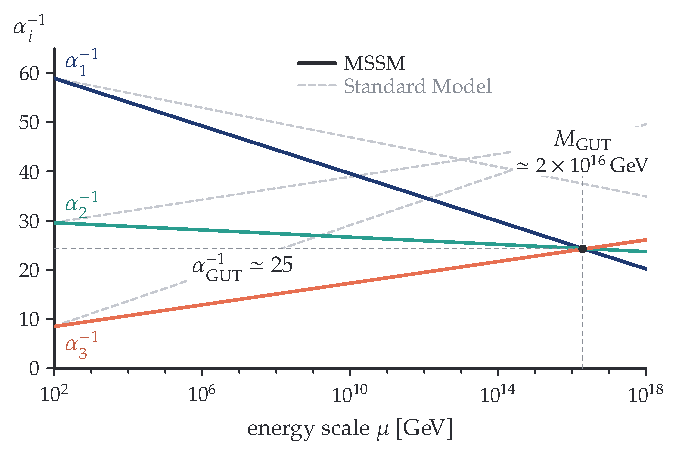
\includegraphics{fig_L2-unification}
  \caption{Running of the three inverse gauge couplings of the Standard Model gauge group with the MSSM spectrum, at one loop. They meet at $\alpha^{-1}_{\mathrm{GUT}}\simeq 25$ at $M_{\mathrm{GUT}}\simeq2\times10^{16}\GeV$.}\label{fig:L2-unification}
\end{figure}

But then \cref{eq:L2-alphaGUT} requires
\begin{equation}
  \Vol \simeq 25\,g_s^2 ,
  \label{eq:L2-V25}
\end{equation}
so one cannot have at the same time $g_s\ll1$ and $\Vol\gg1$, the two conditions of \cref{eq:L1-hierarchy-conditions} for trusting the effective theory. At small string coupling the volume is of order one or smaller, and the higher-derivative ($\alpha'$) corrections are very large; at large volume, where they are suppressed, the string coupling is large, and the loop corrections can never be ignored. Either way it is hard to trust the effective theory. We shall see that type II theories avoid this problem. There the gauge fields live on D-branes, and their coupling is set by the size of the cycle that the branes wrap, not by $\Vol$, so one can go to large volume and small string coupling while keeping $\alpha_{\mathrm{GUT}}^{-1}\simeq25$.

\section{Moduli}
\label{sec:L2-moduli}

The second problem introduces a concept that applies to every string theory, not only to the heterotic string: \emph{moduli stabilisation}. Consider the dimensional reduction of the ten-dimensional metric to four dimensions. Starting from one metric in ten dimensions, one obtains many scalars in four dimensions, the \emph{moduli}. On $X_{10} = \R^{1,3}\times Y_6$ (\cref{eq:L1-X10}), with coordinates $x^\mu$ on $\R^{1,3}$ and $y^m$ on the Calabi--Yau manifold $Y_6$, the metric $G_{MN}(x,y)$ splits into three kinds of components:
\begin{equation}
  G_{MN}(x,y) \longrightarrow
  \begin{cases}
    G_{\mu\nu}(x) , \\[0.5ex]
    G_{\mu m}(x,y) = \sum_I A^I_\mu(x)\,\omega^I_m(y) = 0 \quad\text{for a Calabi--Yau} , \\[0.5ex]
    G_{mn}(x,y) = \sum_I \phi^I(x)\,\omega^I_{mn}(y) .
  \end{cases}
  \label{eq:L2-metric-split}
\end{equation}
The first, with both indices along $\R^{1,3}$, gives the four-dimensional metric. The mixed components $G_{\mu m}$ are four-dimensional vectors, whose zero modes would come from the harmonic one-forms $\omega^I_m(y)$ of $Y_6$, exactly as for $B_{\mu n}$ in \cref{eq:L2-Bmu}. A Calabi--Yau has none ($b_1=0$, \cref{sec:L2-vectors}), so the metric gives no vectors.

The internal components $G_{mn}$ are four-dimensional scalars, since $m$ and $n$ are just labels. They are expanded in scalar fields $\phi^I(x)$ times objects $\omega^I_{mn}(y)$ with two internal indices, and the number of terms is a topological property of $Y_6$: in practice $I$ takes hundreds of values. A metric in ten dimensions therefore gives a metric in four dimensions plus many scalars, which parametrise the internal metric: moving in the space of these fields changes the size or the shape of the Calabi--Yau, as anticipated at the end of \cref{sec:L1-holonomy}. Mathematicians call such parameters of the Calabi--Yau metric moduli; in physics they are scalar fields. One of them is the volume $\Vol$ that appears in $\alpha_{\mathrm{GUT}}$, \cref{eq:L2-alphaGUT}. As a field, $\Vol(x)$ is a function on Minkowski space: the Calabi--Yau attached at the point $x$ can have a different volume from the one attached at another point.

There are, in general, three types of moduli.

\emph{Kähler moduli.} The first type parametrises deformations of the size of $Y_6$; an example is the volume. They are denoted
\begin{equation}
  T_i(x) ,\qquad i = 1,\dots,h^{1,1}(Y_6) ,
  \label{eq:L2-T}
\end{equation}
where $h^{1,1}$, a \emph{Hodge number}, is the number of linearly independent harmonic $(1,1)$-forms on $Y_6$, those annihilated by the Laplacian, $\Delta\omega = 0$: a topological property. The name $(1,1)$ comes from the fact that $Y_6$ is a complex manifold, on which one can use holomorphic and antiholomorphic coordinates $z^i$ and $\bar z^{\bar\imath}$, as one describes the plane either with $(x,y)$ or, as the complex plane, with $(z,\bar z)$. A $(1,1)$-form has one holomorphic and one antiholomorphic index, $\omega_{i\bar\jmath}\,\dd z^i\wedge\dd\bar z^{\bar\jmath}$.

\emph{Complex-structure moduli.} The second type changes the complex structure of $Y_6$, i.e.\ how complex coordinates are assigned to it. Without changing the volume, these deformations change the shape of $Y_6$. They are denoted
\begin{equation}
  U_a(x) ,\qquad a = 1,\dots,h^{2,1}(Y_6) ,
  \label{eq:L2-U}
\end{equation}
where the Hodge number $h^{2,1}$ counts the linearly independent harmonic $(2,1)$-forms on $Y_6$. The beauty of the construction is that topological properties of $Y_6$ correspond to new scalar fields in four dimensions.

\emph{The axio-dilaton.} The third type comes not from the metric but from the other scalars of the massless spectrum of type IIB, \cref{tab:L2-spectra}: the dilaton $\phi$ and the R--R zero-form $C_0$, a scalar since it has no index. They combine into a complex scalar, the \emph{axio-dilaton}
\begin{equation}
  S = e^{-\phi} + i\,C_0 .
  \label{eq:L2-S}
\end{equation}
All the moduli turn out to be complex: $T_i$ and $U_a$, like $S$, are complex scalar fields. The real part of $S$ is $e^{-\phi}$, so by \cref{eq:L1-gs} its expectation value is the inverse string coupling,
\begin{equation}
  \langle\mathrm{Re}\,S\rangle = \frac{1}{g_s} \gg 1 ,
  \label{eq:L2-ReS}
\end{equation}
which must be large for the effective theory to be trusted.

For a typical Calabi--Yau manifold both $h^{1,1}$ and $h^{2,1}$ can be of order $100$, so that one metric in ten dimensions gives hundreds of scalars in four. Calabi--Yau manifolds are named after Eugenio Calabi, an Italian-born mathematician, who conjectured their existence, and Shing-Tung Yau, a Chinese-born mathematician, who proved it; mathematicians and theoretical physicists then started building explicit examples.
Their number is still not known. The largest dataset built so far, that of Kreuzer and Skarke~\cite{KreuzerSkarke}, has about half a billion examples, $473\,800\,776$ (it lists the four-dimensional reflexive polytopes, each of which defines Calabi--Yau threefolds as hypersurfaces in a toric variety), each a good string compactification. A few have both Hodge numbers small, for instance $h^{1,1} = 1$ and a small $h^{2,1}$, and so only a few scalars, but most have many; for the compactification they are all equally good.

\section{The moduli problem}
\label{sec:L2-moduli-problem}

What happens to the physics if there are all these scalars in four dimensions? The answer is that the moduli mediate new interactions. Since in ten dimensions they are the metric, the moduli couple gravitationally to everything. This also explains why we have not seen them: they carry no charge under the Standard Model gauge group, and feel neither QCD nor the electroweak interactions. But the gravitational interaction between two massive particles is the exchange of a graviton, and on top of it there can be the exchange of any of these scalars: a fermion can emit a modulus through a gravitational vertex, and another fermion can absorb it. This is a new interaction of gravitational strength, which modifies Newton's law.

How far can this be tolerated? Newton's inverse-square law $1/r^2$ has been verified experimentally down to distances of a few tens of micrometres, which is not small at all: below that we do not know how gravity behaves, whereas the LHC probes the other interactions down to $10^{-18}\,$m. The reason is that when two bodies are pushed closer to each other the other interactions become more important, and they are hard to shield.
What this means depends on the masses of the moduli. Massless moduli modify gravity at arbitrarily large distances. Massive ones mediate a force of finite range, just as the weak interactions are felt only inside nuclei because the $W$ and $Z$ bosons are massive, and modify gravity only at short distances. To avoid these \emph{fifth forces} a string compactification must give all the moduli a mass large enough for the forces to have escaped detection. At tree level, however, all of them are massless, with nothing to give them a mass, so one has to include quantum corrections and see whether they generate a potential that does. This is the problem of \emph{moduli stabilisation}. A massless field has a flat potential, so its value is not fixed anywhere and can have very large quantum fluctuations; a potential with a minimum stabilises the field there, besides giving it a mass.

In summary, \emph{moduli are uncharged four-dimensional scalars with gravitational-strength interactions with ordinary matter, since they come from the metric, and are massless at leading (tree-level) order in supergravity.} Their potential is flat: deformations of the size and shape of the extra dimensions cost no energy. This would be a phenomenological disaster, for two reasons.

\subsection{Fifth forces}

The first reason is the one just described: massless moduli would mediate fifth forces of Yukawa type, which are not observed. The four-dimensional Lagrangian contains, together with the mass term of a fermion $\psi$ of ordinary matter, such as the electron, an interaction of Yukawa type with a modulus,
\begin{equation}
  \mathcal L_4 \supset \frac{m_\psi}{\Mp}\,\phi\,\bar\psi\psi ,
  \label{eq:L2-yukawa}
\end{equation}
where $\phi$ stands for any of the moduli, canonically normalised, and the coupling up to a coefficient of order one is shown. The suppression by the Planck mass is typical of gravitational interactions. Through this coupling the exchange of $\phi$ between two particles of ordinary matter, \cref{fig:L2-fifthforce}, gives a fifth force, with a vertex $m_\psi/\Mp$ at each end. The observational limit for moduli that couple to ordinary matter with strength $1/\Mp$ is that, to avoid these fifth forces, they must be heavier than about a meV:
\begin{equation}
  m_\phi \gtrsim 1\,\mathrm{meV} .
  \label{eq:L2-bound}
\end{equation}

\begin{figure}[tbp]
  \centering
  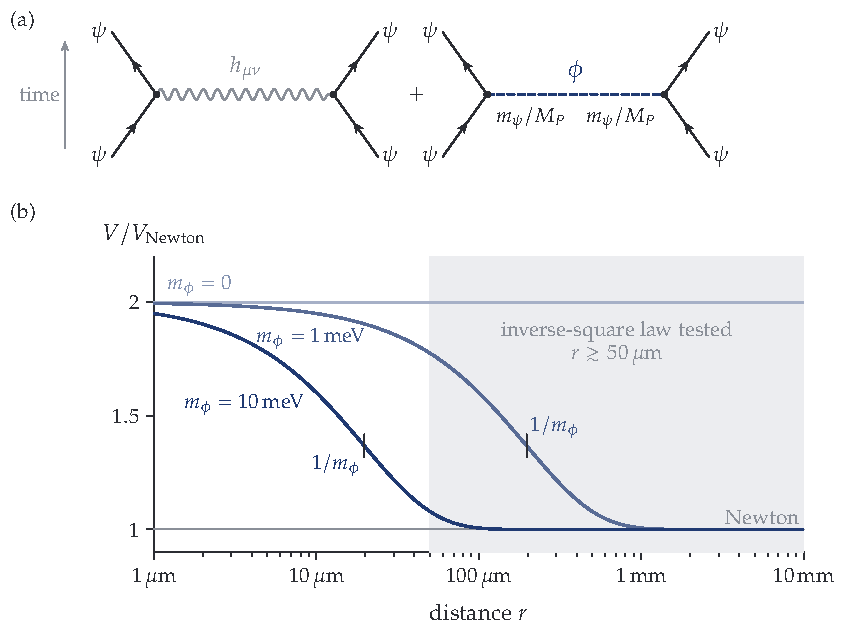
\includegraphics{fig_L2-fifthforce}
  \caption{A modulus as the mediator of a fifth force. (a) Tree-level exchange of a modulus $\phi$ between two fermions, with the coupling of \cref{eq:L2-yukawa} at each vertex, on top of the exchange of a graviton. (b) The resulting potential between two masses relative to Newton's, $V/V_{\mathrm{Newton}} = 1+\alpha_\phi\,e^{-m_\phi r}$, where $\alpha_\phi$ is the strength of the fifth force relative to gravity (here $\alpha_\phi=1$), for a massless modulus and for two massive ones.}\label{fig:L2-fifthforce}
\end{figure}

\subsection{Lack of predictivity}

The second reason is that all the features of the effective theory depend on the moduli. The only parameter that can be fixed by hand is $\alpha'$, and once it is fixed (or traded for $\Mp$, \cref{eq:L1-MP-Ms}) everything else is the vacuum expectation value of a field. For example, the coupling $\alpha_{\mathrm{GUT}}$ of \cref{eq:L2-alphaGUT}, written in terms of the moduli with \cref{eq:L2-ReS}, is
\begin{equation}
  \alpha_{\mathrm{GUT}} \simeq \frac{g_s^2}{\Vol} = \frac{1}{\langle\Vol\rangle\,\langle\mathrm{Re}\,S\rangle^2} ,
  \label{eq:L2-alphaGUT-moduli}
\end{equation}
where $\langle\Vol\rangle$ is the expectation value of the volume modulus: the coupling is the expectation value of a combination of two moduli. If these are massless, their potential is flat, any value is allowed, with huge quantum fluctuations, and $\alpha_{\mathrm{GUT}}$ cannot be predicted. The same holds for the scales of \cref{ch:L1}: the string scale $\Ms\simeq g_s\Mp/\sqrt\Vol$ (\cref{eq:L1-MP-Ms}) and the Kaluza--Klein scale $\MKK\simeq g_s\Mp/\Vol^{2/3}$ (\cref{eq:L1-MKK}) are other combinations of $g_s$ and $\Vol$. Without knowing the moduli one knows neither $\Ms$, nor $\MKK$, nor $\alpha_{\mathrm{GUT}}$: one knows nothing.

There is therefore a huge lack of predictivity, because all the features of the four-dimensional effective theory are functions of the moduli: the gauge couplings, the Yukawa couplings, the mass spectrum, the string and Kaluza--Klein scales, the scale of supersymmetry breaking, the cosmological constant, the scale of inflation, and even the gauge group. In a sense this is the beauty of string theory, since all these quantities can be predicted rather than chosen by hand; but with massless moduli nothing is predicted.

What is needed is \emph{moduli stabilisation}: the study of the quantum corrections to the scalar potential $V$ (not to be confused with the volume $\Vol$), which can develop a minimum, stabilise the moduli $\phi^I$ there, make them massive and fix the predictions,
\begin{equation}
  \frac{\partial V}{\partial\phi^I}\bigg|_{\langle\phi\rangle} = 0 ,\qquad
  m^2_{IJ}\propto\frac{\partial^2V}{\partial\phi^I\partial\phi^J}\bigg|_{\langle\phi\rangle}\ \text{positive definite} ,
  \label{eq:L2-stabilisation}
\end{equation}
with the mass matrix normalised by the kinetic terms of the moduli, and with masses large enough to satisfy \cref{eq:L2-bound} and the much stronger cosmological bound \cref{eq:L3-CMP-bound} of \cref{sec:L3-CMP}. Why this is hard in the heterotic string is the subject of \cref{sec:L3-heterotic}; a hint is already in \cref{sec:L2-alphaGUT}: there the quantum corrections are hard to control, and yet they are exactly what is needed to stabilise the moduli.
